\documentclass[8pt,aspectratio=169]{beamer}
\usetheme{Boadilla}


\usepackage[utf8]{inputenc}
\usepackage{dsfont}

\usepackage{hyperref}
\usepackage{graphicx}
\usepackage{caption}
\usepackage{subcaption}
%\usepackage{amsmath,amssymb,physics}

\usepackage{amsmath, amssymb, amscd, amsfonts, mathtools, physics, hyperref, color}

\usepackage{tikz}

% Set beamer color info
\definecolor{BIBlue}{RGB}{0,50,150}
\setbeamercolor{title}{fg=black}
\setbeamercolor{frametitle}{fg=black}
\setbeamercolor{structure}{fg=BIBlue}


%Stolen from https://tex.stackexchange.com/questions/388344/beamer-adding-some-text-in-subsection-title-page
\setbeamertemplate{section page}
{
    \begingroup
    \begin{beamercolorbox}[sep=10pt,center,rounded=true,shadow=true]{section title}
        \usebeamerfont{section title}\insertsection\par
    \end{beamercolorbox}
    \endgroup
}

\title{Diversity with Similarity as a Measure of Training Set Quality}
\institute{
    Beth Israel Deaconess Medical Center\\
}

\author{
    Josiah Couch\\
    }
\subtitle{
    based on 2407.15724
    }
%\institute{Beth Israel Deaconess Medical Center}
\date{13 August 2024}



\begin{document}

\begin{frame}
\titlepage
\end{frame}

%\begin{frame}
%\frametitle{Outline}
%\tableofcontents[]
%\end{frame}

\section{Introduction}
%\begin{frame}
%\sectionpage
%\end{frame}


\begin{frame}
\frametitle{Motivation}

\onslide<1->{
\begin{minipage}[t]{0.45\linewidth}

    \begin{itemize}
        \item \onslide<2->{We want to understand training set quality}
        \begin{itemize}
            \item \onslide<3->{high quality training set $\rightarrow$ high performance model}
            \item \onslide<4->{(We can take this as the definition))}
        \end{itemize}
        \item \onslide<5->{In particular, what features diagnose a dataset as high quality?}
        \begin{itemize}
            \item \onslide<6->{Class balance and size (obviously)}
            \item \onslide<7->{Dataset diversity}
            \begin{itemize}
                \item \onslide<8->{Class internal diversity}
                \item \onslide<9->{Overall diversity}
            \end{itemize}
        \end{itemize}
        \item \onslide<10->{How does one measure training set diversity?}
        \begin{itemize}
            \item \onslide<11->{The (exponential of) entropy provides a natural notion of diversity}
            \item \onslide<12->{We will use a deformation of the entropy which accounts for similarities}
            \item \onslide<13->{To account for both class internal and overal diversity, we will consider the entropy of the joint distribution on features + classes}
        \end{itemize}
    \end{itemize}

\end{minipage}}
%
\hfill
%
\begin{minipage}[t]{0.45\linewidth}
\onslide<1->{
    \begin{figure}
        \begin{center}
        
        \begin{subfigure}[b]{0.2\textwidth}
             \centering
             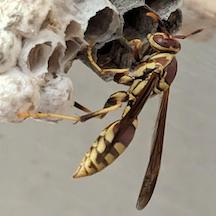
\includegraphics[width=\textwidth]{slide_img/wasp1.jpeg}
         \end{subfigure}   
         %
        \begin{subfigure}[b]{0.2\textwidth}
             \centering
             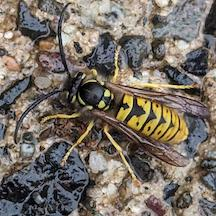
\includegraphics[width=\textwidth]{slide_img/wasp2.jpeg}
         \end{subfigure}
         %
        \begin{subfigure}[b]{0.2\textwidth}
             \centering
             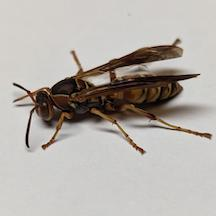
\includegraphics[width=\textwidth]{slide_img/wasp3.jpeg}
         \end{subfigure} 
         %
        \begin{subfigure}[b]{0.2\textwidth}
             \centering
             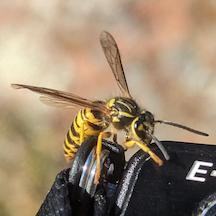
\includegraphics[width=\textwidth]{slide_img/wasp6.jpeg}
         \end{subfigure} 
         
        \begin{subfigure}[b]{0.2\textwidth}
             \centering
             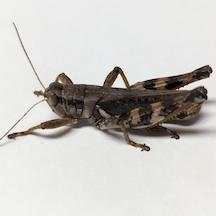
\includegraphics[width=\textwidth]{slide_img/grasshopper3.jpeg}
         \end{subfigure}   
         %
        \begin{subfigure}[b]{0.2\textwidth}
             \centering
             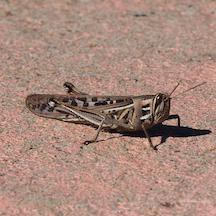
\includegraphics[width=\textwidth]{slide_img/grasshopper4.jpeg}
         \end{subfigure}
         %
        \begin{subfigure}[b]{0.2\textwidth}
             \centering
             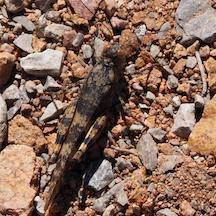
\includegraphics[width=\textwidth]{slide_img/grasshopper5.jpeg}
         \end{subfigure}
         %
        \begin{subfigure}[b]{0.2\textwidth}
             \centering
             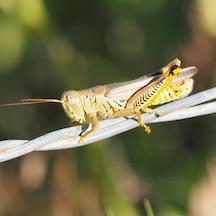
\includegraphics[width=\textwidth]{slide_img/grasshopper6.jpeg}
         \end{subfigure}
        
        \end{center}
        \caption{A high diversity dataset}
    \end{figure}


    \begin{figure}
        \begin{center}
        \begin{subfigure}[b]{0.2\textwidth}
             \centering
             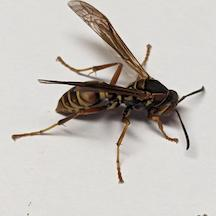
\includegraphics[width=\textwidth]{slide_img/wasp4.jpeg}
         \end{subfigure}   
         %
        \begin{subfigure}[b]{0.2\textwidth}
             \centering
             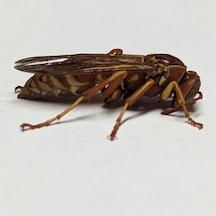
\includegraphics[width=\textwidth]{slide_img/wasp5.jpeg}
         \end{subfigure}
         %
        \begin{subfigure}[b]{0.2\textwidth}
             \centering
             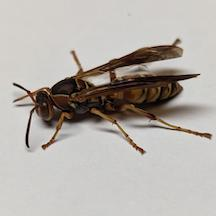
\includegraphics[width=\textwidth]{slide_img/wasp3.jpeg}
         \end{subfigure}
         %
        \begin{subfigure}[b]{0.2\textwidth}
             \centering
             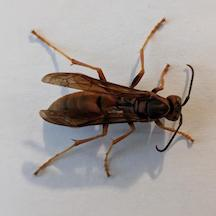
\includegraphics[width=\textwidth]{slide_img/wasp7.jpeg}
         \end{subfigure}
         
        \begin{subfigure}[b]{0.2\textwidth}
             \centering
             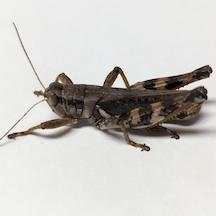
\includegraphics[width=\textwidth]{slide_img/grasshopper3.jpeg}
         \end{subfigure}   
         %
        \begin{subfigure}[b]{0.2\textwidth}
             \centering
             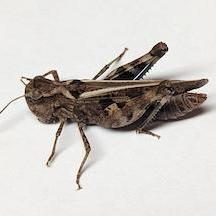
\includegraphics[width=\textwidth]{slide_img/grasshopper2.jpeg}
         \end{subfigure}
         %
        \begin{subfigure}[b]{0.2\textwidth}
             \centering
             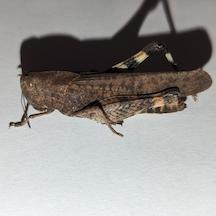
\includegraphics[width=\textwidth]{slide_img/grasshopper1.jpeg}
         \end{subfigure}
         %
        \begin{subfigure}[b]{0.2\textwidth}
             \centering
             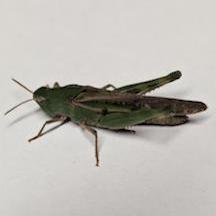
\includegraphics[width=\textwidth]{slide_img/grasshopper7.jpeg}
         \end{subfigure}
        
        \end{center}
        \caption{A low diveristy dataset}
    \end{figure}
}
\end{minipage}

\end{frame}

\subsection{Diversity with Similarity}
\begin{frame}
\frametitle{Diversity with Similarity}

\begin{itemize}
    \onslide<2->{\item The exponentials of the R\'enyi entropies (the \textit{Hill numbers} \cite{hill1973}) have long been used to quantify diversity
    \begin{equation}
        D_q(p) = e^{H_q(p)} \text{; } H_q(p) = - \frac{1}{q-1} \log \sum_i p^q = - \frac{1}{q-1} \log \expval{p^{q-1}}_p
    \end{equation}}
    \onslide<3->{\item E.g. in ecology}
    \onslide<4->{\item However, these measures fail to capture the following intuition: }
    \begin{itemize}
        \onslide<5->{\item Given two communities each consisting of $N$ uniformly distributed species, if the first consists of only species from the same genus, and the second consists of species from more than one genus, the second should be more diverse!}
        \onslide<6->{\item This is still ture if I replace 'genus' with some higher taxanomic unit and 'species' by some relatively lower unit (e.g. family and genus)}
    \end{itemize}
        
\end{itemize}

\begin{figure}
    \centering
    
\includegraphics[width=0.7\linewidth]{slides/slide_img/animals.pdf}
    \caption{Nine species of birds are less diverse than nine species drawn from across the animal family tree}
    \label{fig:animals}
\end{figure}

\end{frame}

\begin{frame}
\frametitle{Diversity with Similarity (continued)}

\onslide<1->{To remedy this deficit, one may define\cite{leinster2012}:}

\begin{itemize}
    \onslide<2->{\item A similarity matrix $Z_{ij}$ whose $ij$th entry encodes the similarity between species $i$ and species $j$}
    \onslide<3->{\item The similarity deformed R\'enyi entropy,
    \begin{equation}
        H_q^Z(p) = - \frac{1}{q-1} \log \expval{(Zp)^{q-1}}_p = - \frac{1}{q-1} \log \sum_i p_i \left(\sum_j Z_{ij} p_j \right)^{q-1}
    \end{equation}}
    
    \onslide<4->{\item The corresponding similarity sensitive diversity $D_q^Z(p) = e^{H_q^Z(p)}$}
    
    \onslide<5->{\item N.B. that when $Z$ is the identity matrix, these reduce to the ordinary R\'enyi entropies/Hill numbers.}
    
    \onslide<6->{\item Also, even though we defined a similarity matrix on species, w.l.o.g. we could have defined a similarity matrix on individuals.}
    
\end{itemize}

\onslide<7->{In our context (ML for medical imaging)}

\begin{itemize}
    \item \onslide<8->{ Each image is considered a unique species}
    \item \onslide<9->{ For simplicity, the similarity is chosen to be $Z(x,y) = \exp(-d_{RMSD}(x,y))$, where $d_{RMSD}$ is the pixel-wise root mean squared difference}
\end{itemize}



\end{frame}

\begin{frame}
\frametitle{Metacommunity and subcommunity}

\begin{minipage}[t]{0.4\linewidth}
\begin{itemize}
    \onslide<2->{\item In many situation, one may want to compare diversity of parts to that of the whole}
    \begin{itemize}
        \onslide<3->{\item E.g. in ecology, islands vs a whole island chain}
        \onslide<4->{\item E.g. in ML, training set vs individual classes}
    \end{itemize}
    \onslide<5->{\item For this purpose, one may label each individual both by species/type and by subcommunity, and consider the joint distribution \cite{leinster2012, reeve2016}}
    \begin{itemize}
        \onslide<6->{\item The exponential of the entropy of the joint distribution is then termed the \textit{Alpha diversity}}
        \onslide<7->{\item The exponential of the mutual information between species and subcommunity is termed (normalized) \textit{Beta diversity}}
        \onslide<8->{\item That of the marginal distribution on species/subcommunity are termed \textit{Gamma/Delta diversity}}
    \end{itemize}
    \onslide<9->{\item All of this goes through when considering a similarity on species (we won't consider a similarity on subcommunities)}
\end{itemize}
\end{minipage}
%
\hfill
%
\begin{minipage}[t]{0.5\linewidth}
\begin{eqnarray}
    A^Z_q (p) &=& \left[ \sum_{i,\mu} p(x_i, y_\mu) \left( \sum_{j} Z_{ij} p(x_j, y_\mu) \right)^{q-1} \right]^{1-q}\\
    B^Z_q (p) &=& \left[ \sum_{i,\mu} p(x_i, y_\mu) \left( \frac{\sum_j Z_{i,j} p(x_j, y_\mu)}{\sum_j Z_{ij} p(x_j) p(y_\mu)} \right)^{q-1} \right]^{1-q}\\
    \Gamma^Z_q (p) &=& \left[ \sum_{i} p(x_i) \left( \sum_{j} Z_{ij} p(x_j) \right)^{q-1} \right]^{1-q}\\
    \Delta^Z_q (p) &=& \left[ \sum_{\mu} p(y_\mu)^q \right]^{1-q}
\end{eqnarray}
\end{minipage}
    
\end{frame}

\section{Methodology}
%\begin{frame}
%\sectionpage
%\end{frame}

\begin{frame}
\frametitle{Methodology}

\begin{minipage}[t]{0.55\textwidth}
\begin{enumerate}
    \item \onslide<2->{Collect a number of datasets}
    \begin{itemize}
        \item \onslide<3->{PathMNIST, BloodMNIST, OrganAMNIST, and OrganCMNIST from MedMNIST \cite{medmnistv1, medmnistv2}}
        \item \onslide<4->{Several additional datasets, including those used in Madani et al. \cite{madani2018} and Chinn et al. \cite{Chinn2021}}
    \end{itemize}
    \item \onslide<5->{From each dataset, sample the training set to create many subsets}
    
    \item \onslide<6->{Train classifier on each subset}
    
    \item \onslide<7->{Test each of these models against test set (common to subsets from a given source)}
    
    \item \onslide<8->{Measure an assortment of diversity indices for each subset (including class balance)}
    
    \item \onslide<9->{Use linear regression to measure how much variation in model performance is explained by different sets of diversity indices.}
    
    \onslide<10->{\item (Our models are actually log linear, and each model includes the image size, number of color channels, and number of classes as features)}
    
\end{enumerate}
    
\end{minipage}
%
\begin{minipage}[t]{0.35\textwidth}

\begin{figure}
    \centering
    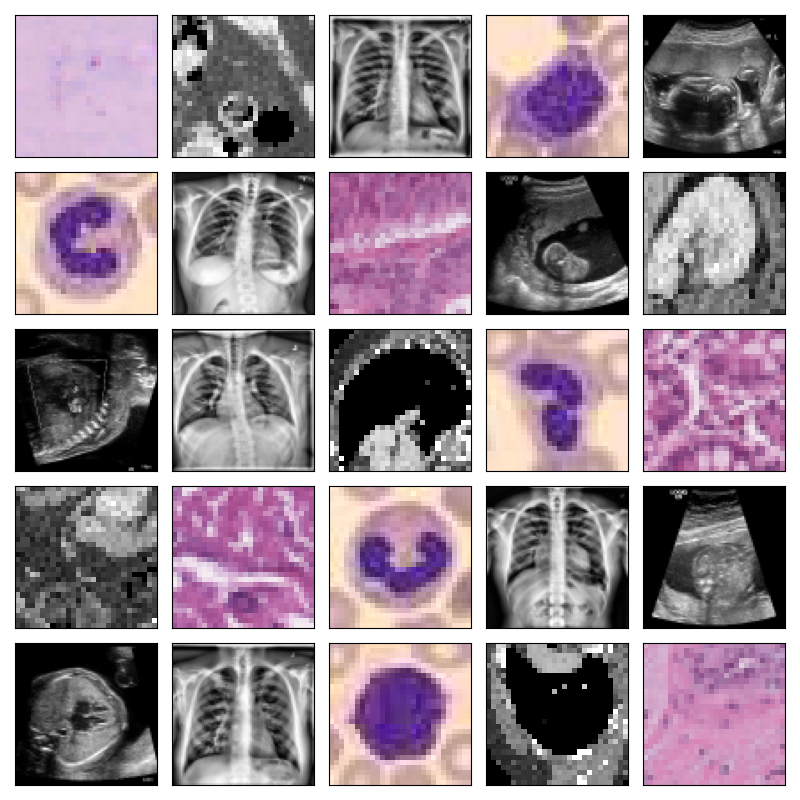
\includegraphics[width=0.9\textwidth]{slide_img/image_grid.png}
    \caption{Images from some of the selected datasets}
\end{figure}

\end{minipage}
    
\end{frame}

\begin{frame}
\frametitle{Results}

We found that some diversities with similarity, especially the Alpha diversity (at R\'enyi parameters $0$ and $1$), outperform class balance, both singly and when combined with size.

\begin{figure}
    \centering
    \begin{subfigure}[b]{0.25\textwidth}
         \centering
         
\includegraphics[width=\textwidth]{slides/slide_img/results_a.png}
     \end{subfigure}
    \begin{subfigure}[b]{0.28\textwidth}
         \centering
         
\includegraphics[width=\textwidth]{slides/slide_img/results_b.png}
     \end{subfigure}
    \caption{$R^2$ for linear models of resnet-18 accuracy trained on different sets of diversities (a) single features (b) pairs of features}
    \label{}
\end{figure}
    
\end{frame}

\begin{frame}
\frametitle{Acknowlegements}

%\begin{center}

I'd like to thank IAIFI for hosting this workshop, as well as my collaborators, Dr. Ramy Arnaout (BIDMC and HMS) and Dr. Rima Arnaout (UCSF Department of Medicine). This work was supported by the Gordon and Betty Moore foundation and by the NIH.



\begin{figure}
    \centering
    
\includegraphics[width=0.2\linewidth]{slides/slide_img/QR_code_arxiv.png}
    \caption{Link to paper: \url{https://arxiv.org/abs/2407.15724}}
    \label{fig:QR}
\end{figure}

\vspace{0.02\textwidth}

Thank you for attending my talk!
    
%\end{center}
    
\end{frame}

\begin{frame}
\frametitle{References}
{\tiny
\bibliographystyle{JHEP} %JHEP.bst
\footnotesize\bibliography{main}
}
\end{frame}

\end{document}
